\chapter{Structure learning}\label{chp:structure}

In this chapter we cover two structure learning algorithms we use for image classification. The
first is based on~\cite{clustering}. The second is a variation of~\cite{gens-domingos}'s structure
learning schema. Once we cover both algorithms, we explain how we add a slight modification to the
first architecture. We have empirically found that this change increased image classification
accuracy significantly. We call this the ``classification architecture''.

\section{The Dennis-Ventura architecture}\label{section:dv}

Let us first formalize the notion of dataset. We call a dataset a set of \textit{instances}, where
each instance is a set we call \textit{valuation} or \textit{instantiation}. As we have mentioned
before, a valuation may be incomplete, meaning that an instantiation of some random variable may be
missing from the instance. In this thesis we assume complete data, as both structure learning
algorithms do not admit incomplete datasets.

Having said that, let $D$ be a complete dataset. Since $D$ is complete, for each instance $I$ we
can map each random variable $X$ from $I$ to a number, yielding an ordered vector $(X_1,X_2,\ldots,
X_m)$ equivalent to $I$. We do the same for each instance $I$. The vector $(I_1,I_2,\ldots, I_n)$
is a representation of $D$. This way, $D$ could be seen as a $m\times n$ matrix. We denote by
$D^\intercal$ the transpose of the matrix representation of the dataset $D$.  Let $T$ be a
subscope, that is, a subset of the set of all variables in the SPN\@. We use the notation $D_T$ to
represent the matrix of all instances from $D$ but restricted only to elements from random
variables in $T$.

Since we are restricted to the image classification domain, we give some semantic meaning to
datasets. If $D$ is a dataset, then each instance $I\in D$ can be seen as a vector containing all
the pixel values of an image plus a classification label. Each variable is a pixel from the image,
and each variable value is the pixel's color intensity. If the dataset $D$ is a vector of images
and their labels, the transpose $D^\intercal$ is a vector of variables and their values in each
image.

Just like in~\cite{poon-domingos}, the Dennis-Ventura algorithm uses the notion of similarity
between local variables.  This local neighborhood is called a Region. A Region represents a cluster
of pixels that has some semantic value when grouped together. Contrastingly, a Decomposition
represents independence between variables. In an SPN, a Region is graphically represented by a set
of sum nodes, whilst a Decomposition is a set of products.

To learn an SPN structure from data,~\cite{clustering} uses a \textit{region graph}, which is a
simplified representation of an SPN made out of Region nodes and Decomposition nodes.

\begin{figure}[h]
  \begin{subfigure}{.4\linewidth}
    \centering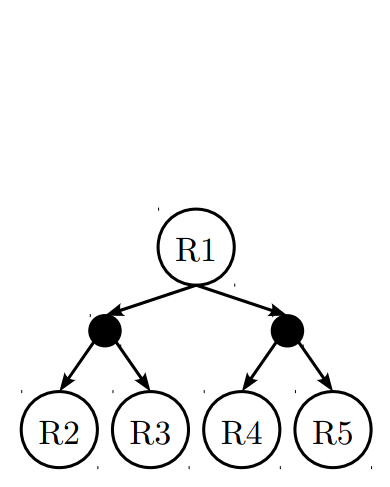
\includegraphics[scale=1.0]{imgs/simple_dv.png}
    \caption{}
  \end{subfigure}
  \begin{subfigure}{.6\linewidth}
    \centering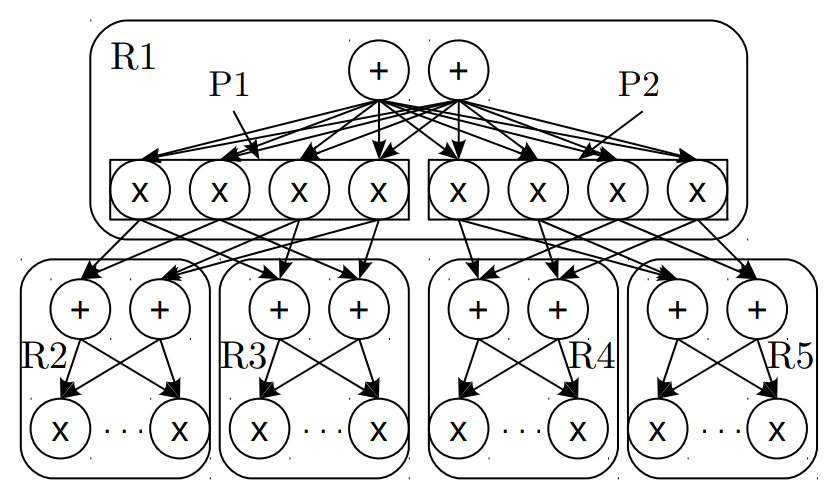
\includegraphics[scale=1.0]{imgs/trans_dv.png}
    \caption{}
  \end{subfigure}
  \caption{Dennis-Ventura region graph and translated SPN as shown in~\cite{clustering}.}
\end{figure}

The region graph is generated by recursively finding two subregions from a parent region through
the use of $k$-means clustering. Let $R$ be a region, and $D_R^\intercal$ the transposed dataset
restricted to $R$'s scope. We partition $R$ into two subregions $R_1$ and $R_2$ by $k$-means
clustering $D_R^\intercal$, yielding two subclusters $D_{R_1}^\intercal$ and $D_{R_2}^\intercal$.
We then apply recursion on the two subregions. At each clustering step, we connect regions $R$ to a
decomposition node $P$, which is then connected to each $R_i$ node. Our stop criteria is when
$\Sc(R_i)=1$. The root node is a special case. We run $k$-means cluster on $D$, and for each
$D_i$ cluster, we construct a sub-SPN for each root child with $D_i$.

Once created, the region graph is then translated to a valid SPN\@. Each region node $R$ is
translated to a set of SPN nodes. If $\Sc(R)=1$, then these nodes are $g$ univariate gaussian
distributions, where each gaussian is a different quantile of the distribution of the pixel. Else,
$m$ sum nodes are created. Partition nodes are translated to product nodes. Edges are added such
that every product child node of a region is connected to all sum nodes in the region. Each of
these product nodes are then connected to a distinct pair of sum nodes from both region's children
subregions, meaning that each decomposition node contains $2^m$ products.

With the architecture done, we apply parameter learning on the SPN to learn weights. This is done
either through gradient descent or EM\@. In this thesis we apply generative and discriminative
gradient descent to the architecture.

\section{The Gens-Domingos schema}\label{section:gd}

In~\cite{gens-domingos}, Gens and Domingos describe a flexible schema for structure learning of
SPNs. The schema is based on the idea that the scope in a sum node's child mean that these
variables are similar (and by consequence dissimilar to the variables in other sibling nodes'
scopes), and that variables in a product's child mean that variables are dependent of each other
(and analogally to sums, independent of other siblings).

This interpretation of SPNs yields an adaptable and open schema of learning. Sum nodes are created
through clustering, as each cluster has some similarity aspect given some metric. Meanwhile,
product nodes are created through statistical variable independence algorithms. When the scope of
this partitioning of variables is one, we create a univariate distribution over the partitioned
dataset.

\begin{algorithm}[H]
  \caption{\code{GensArch}: Gens-Domingos structure learning schema}
  \begin{algorithmic}[1]
    \Require Set of instances $D$ and scope $X$
    \Ensure SPN structure learned from $D$ and $X$
    \If{$|X|=1$}
      \State \textbf{return} univariate distribution over $D_X$
    \Else%
      \State Partition $X$ into $P_1,P_2,\ldots,P_m$ such that every $P_i$ is independent of $P_j$,
        $i\neq j$
      \If{$m>1$}
        \State Let $\pi$ be a new product node
        \For{$i\gets 1,\ldots,m$}
          \State $p_i\gets$\code{GensArch}$(D_{P_i}, P_i)$
          \State $\pi$\code{.AddChild}$(p_i)$
        \EndFor%
        \State \textbf{return} $\pi$
      \Else%
        \State Cluster $D$ such that $Q_1,Q_2,\ldots,Q_n$ are $D$'s clusters
        \State Let $\sigma$ be a new sum node
        \For{$i\gets 1,\ldots,n$}
          \State $s_i\gets$\code{GensArch}$(Q_i, X)$
          \State $w\gets |Q_i|/|D|$
          \State $\sigma$\code{.AddChild}$(s_i, w)$ \Comment{$w$ is edge $\sigma\to s_i$'s weight}
        \EndFor%
        \State \textbf{return} $\sigma$
      \EndIf%
    \EndIf%
  \end{algorithmic}
\end{algorithm}

Our implementation was done by using DBSCAN, a density based clustering algorithm that
automatically decides the number of clusters to generate (\cite{dbscan}), for clustering and the
traditional G-test for variable independence. We also implemented $k$-means, $k$-mode and
$k$-median for clustering and Pearson's $\chi^2$-square for independence testing. We found that
DBSCAN yielded the best accuracy results on clustering, but took a long time for training. Using
$k$-means clustering with $k=2$ yielded worse, but comparable results, but with the upside of being
fast to train. The G-test provided the best variable independence results.

Finding independent variable subsets can be done by iteratively comparing variables pairwise. The
connected components of the resulting disconnected graph are independent subsets. This brute force
approach is intractable, as the G-test already takes $\bigo(|X||Y|)$ time, where $X$ and $Y$ are
random variables and $|\cdot|$ indicates the number of categories of the RV, and testing each pair
of variables exhaustively is exponential.

Instead of testing every variable pairwise, we constructed a dependency graph. Each vertex from the
dependency graph represents a variable. An edge between two vertices means the two variables are
dependent. To find independent partitions in a dataset it suffices to find a spanning tree of the
dependency graph. We do this through Kruskal's MST union-find algorithm. The resulting connected
components of the spanning tree are the partitions we wish to find. This significantly reduces
complexity. However, we have found that it still accounts for approximately 90\% of the algorithm's
runtime.

We speculate that a better approach to variable indepedence would be finding approximate spanning
trees on the graph. Many independence tests resulted in a completely dependent graph, but with
cuts that could possibly yield better accuracy and runtime performance.

Our Gens-Domingos implementation generated very deep and expressive SPNs, resulting in good
accuracy results. However, the algorithm only generates SPTs, as once each step (either clustering
or variable independence) is concluded, the function never returns to the same node.

\section{The classification architecture}

The Dennis-Ventura structure learning algorithm is able to model classification problems by
partitioning data into $l$ clusters, where $l$ is the total number of labels, and assigning a
sub-SPN for each cluster. One can interpret each sub-SPN as a model of each label. However,
clustering may not select the right classification instances for each label, as we have no control
over which labels fit each cluster. This effect is intensified on datasets containing a large
number of data.

We try to solve this problem by simplifying the model. Instead of generating sub-SPNs through
clustering, we restrict each label to its own SPN\@. In our architecture, we create a single sum
node as root, representing the image and its classification label. For each label $l$, we construct
a sub-SPN $S_l$ such that the SPN is still valid. This is done by assigning a product node as
$S_l$'s root. Let $Y$ be the classification variable. Each of these products are then connected to
an indicator variable $[Y=y_l]$ and a sub-SPN restricted to only data where $Y=y_l$.

\begin{figure}[h]
  \centering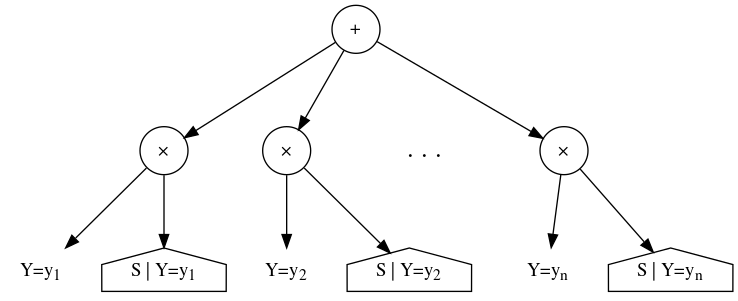
\includegraphics[scale=0.5]{graphs/classarch.png}
  \caption{The classification architecture for the Dennis-Ventura structure.\label{fig:class_arch}}
\end{figure}

\autoref{fig:class_arch} shows the graphical representation of the classification architecture. The
SPN is still valid, as the product node guarantees decomposability and the root sum node is
complete. Each sub-SPN $S|Y=y_i$ is then constructed with the Dennis-Ventura algorithm, but
restricted to data with the $Y=y_i$ valuation.

In practice, this architecture yielded much better results than the original clustering method.
Furthermore, it is possible to easily parallelize each $S|Y=y_i$ learning procedures for faster
learning runtime. Similarly, since each $S|Y=y_i$ is independent of other restricted SPNs, we can
compute SPN values concurrently, allowing for faster inference. We cover this more thoroughly
in~\autoref{chp:modelling}.

Interestingly, when this architecture model was applied to the Gens-Domingos algorithm, accuracy
decreased. This is possibly due to the limitations of trees in SPNs. Another possible reason is
that the Gens-Domingos better captures interactions between labels and pixels than only between
pixels.
